%\definecolor{MyGreen}{rgb}{.13,.55,.13}%{0,1,0} 
%\settikzpagecorners
In this section, we discuss the basics of Matlab.

\section{Matlab: Introduction}\label{sec:Matlab_introduction}

There are many different software packages available.  It's important to understand the different capabilities of each as one software package may be the best tool depending on the task.
Here, we introduce Matlab, which stands for MATrix LABoratory.  Matlab is cost-effective, easy to learn and blends powerful number crunching capabilities with graphical display.  It is an excellent tool for working with large data sets.

Other packages that you may wish to consider, include Mathematica, Maple, Fortran, C, C++, or Java.  In some cases, even a basic TI calculator or Excel is the appropriate tool.

Matlab has become the industry standard for use in many fields including Mathematics, Bioinformatics, Finance, and Engineering.  The basic Matlab package includes the core package and Simulink, a platform for modeling dynamic systems.  Matlab can also be enhanced through the addition of ``toolboxes'' (available from Mathworks) including such topics as Control Systems, Image Processing, Splines and SimBiology. 

\section{Matlab: Layout}\label{sec:Matlab_layout}

We now take a look at the (default) layout of Matlab:


\hspace{-.25in}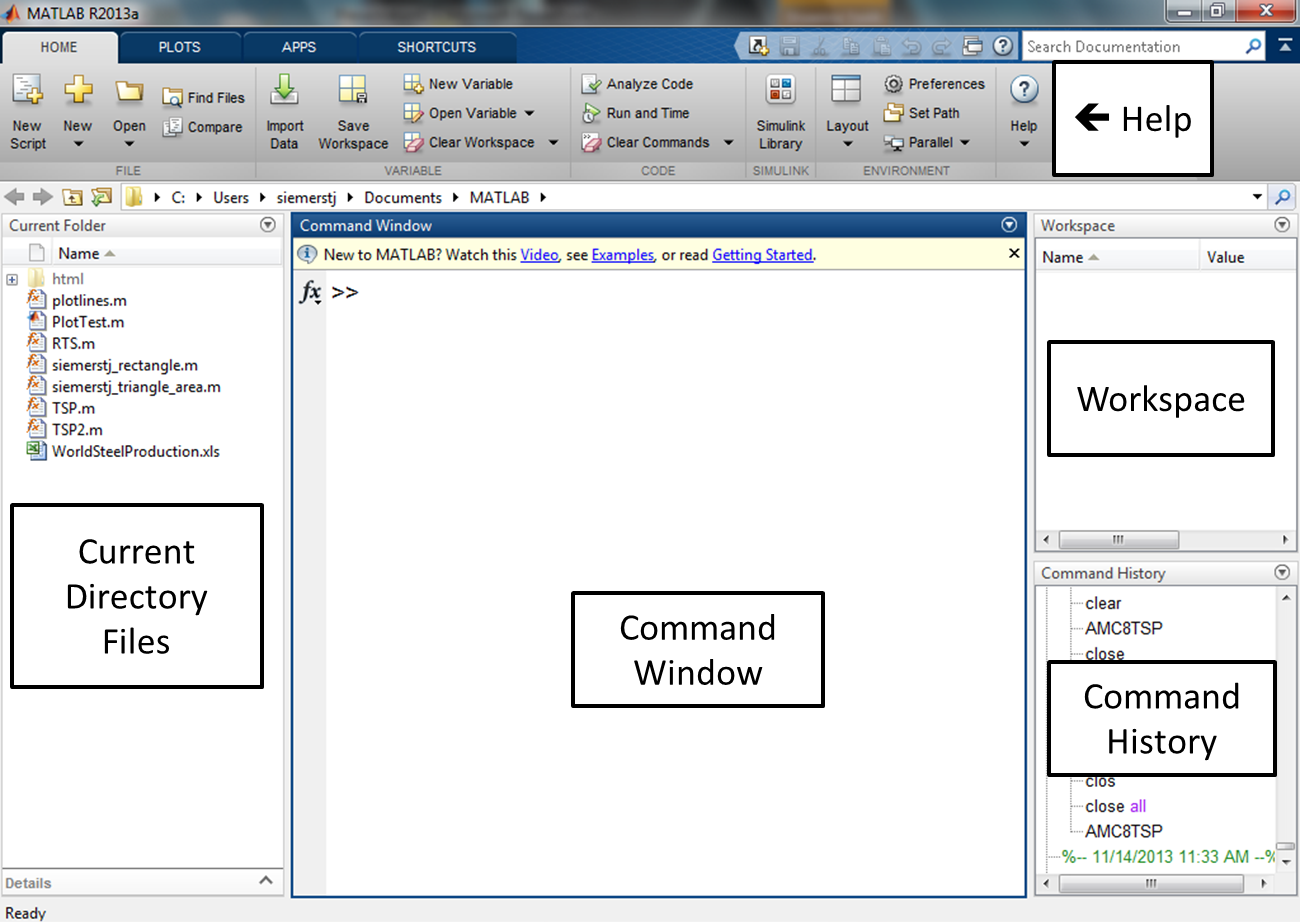
\includegraphics[scale=.55]{figures/matlab_layout2.png}


You can customize how the layout appears, but there are a few main components:\\

\index{Matlab!Command Window}
\noindent \large \textsf{\textbf{Command Window}} \normalsize\\

The command window is where you can perform basic calculations, enter commands, run programs, and view the numeric output.\\

\index{Matlab!Command History}
\noindent \large \textsf{\textbf{Command History}} \normalsize\\

The command history keeps a record of past commands that were entered in the command window.  To run a command again from the command history, you can simply double click it.  Or, if you want to alter the command before running it, you can click and drag it to the command window, change it and then run it (by hitting Enter).\\

\noindent \large \textsf{\textbf{Directory and Workspace (in tabs)}} \normalsize\\


The directory shows the files in the current directory (which itself is listed at the top of the screen).  These files can be run by double clicking, or by clicking and dragging them into the command window.  The workspace keeps track of the variables that are created.  Double clicking a variable in the workspace opens a spreadsheet where the variable can be altered.\\

\newpage
\index{Matlab!Directory}
\noindent \large \textsf{\textbf{Current Directory}} \normalsize\\

When you run any program, it is important that your Current Directory is set to the location of your program.  You can also run programs in a different directory by setting the ``path'' to that directory.  To keep it simple, we will not explain how to do this here, but refer you to the help files.\\

\index{Matlab!Built-in Help}
\noindent \large \textsf{\textbf{Help}} \normalsize\\

The help capabilities in Matlab are well documented.  It does take some time to understand Matlab syntax, but if a user is familar with another programming language, the commands are easy to pick up.  Functions in Matlab are also well named, so you can often guess the name of a function that you may need.


\section{Matlab: Command Window Examples}\label{sec:Matlab_command_window_examples}

Let's try some basic examples in the command window. Enter 5+5 in the command window (and press Enter)\\
\\
\cour{>> 5+5}\\
\cour{ans $=$}\\
\cour{\ps 10}\\

The value 10 has been assigned to the variable \cour{ans}. Next, try the following\\
\\
\cour{>>a=5+5}\\
\cour{a=}\\
\cour{\ps 10}\\
\\
\cour{>>b=5+5; \color{mygreen} \% the semicolon suppresses output.}\\
\index{Matlab!semicolon (;)}

A few things to note.  First, assignment of values to the variables is �right to left� (whatever is on the right of the equals sign is assigned to the variable on the left).  Here, both both \cour{a} and \cour{b} are equal to 10, but only \cour{a}'s value is displayed because the semicolon is used to suppress the output to the screen.  This is a very useful tool in programs where, for example, you want to hide the intermediate calculations.

While there are thousands of commands in Matlab, here are a few that you will use often:\\

\index{Matlab Functions!\cour{clc}}
\index{Matlab Functions!\cour{clear}}
\index{Matlab Functions!\cour{close}}
\index{Matlab Functions!\cour{ctrl + c}}
\noindent \cour{clc} � clears the command window\\
\cour{clear {\color{myred} all}} � clears all the variables\\
\cour{clear {\color{myred} variablename}} � clears the variable named \cour{variablename}\\
\cour{close {\color{myred} all}} � closes all open plot windows\\
\cour{ctrl + c} � stops a running process (important later!)\\

There are several rules about the naming of variables (look those up in Help or Google), but in particular, all variable names must start with a letter and all variables are case sensitive (upper case and lower case letters are considered different)!!  So, for example, the variables \cour{Math} and \cour{math} are treated as different variables.

One final ``peculiar'' aspect of Matlab, is that you can only edit the line you are on!!
You can however recall previous commands with the up and down arrow keys, or type text and use the up and down arrow keys to scroll through the commands starting with that text.

\index{Matlab!Editor}
\section{Matlab: Editor}\label{sec:Matlab_editor}

It is tedious to type everything into the command window, not to mention trying to fix any errors.  We now look at the \textbf{Editor}, where you will write your Matlab \textbf{script files} (basic programs) and \textbf{function files} (user-defined functions).  

As with many aspects of Matlab, there are usually many ways to perform a task.
To start the Editor window, you can either type \cour{edit} in the command window or you can click on the ``new script'' button 

\includegraphics[scale=.5]{figures/matlab_editor_button2}.

The Editor is shown below.  In the blue bar at the top of this image, you can see that the file is currently Untitled.  The asterisk indicates that the file has not been saved since the last change to the file.  Try entering the text exactly as shown.\\

\hspace{-.25in}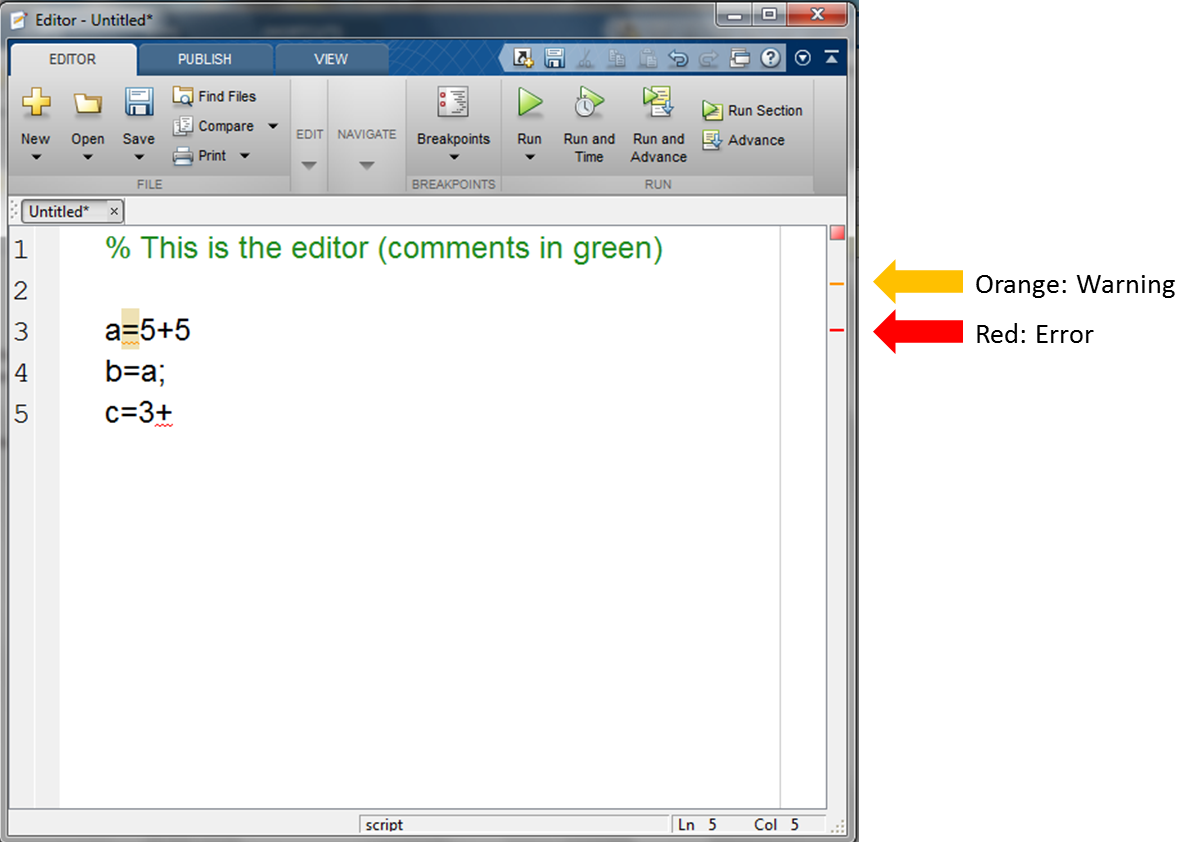
\includegraphics[scale=.6]{figures/matlab_editor2}\\

There are few more key parts to this file.  Any text that follows a percent sign (\cour{\color{mygreen}\%}) is a \textbf{comment} and is colored green.  These are ignored when the program is actually run, but are an important part of the documentation of the file.  It is crucial that you document your files properly both to remind yourself what parts of the program do and to inform any other users that may work with the program in the future.

As you type lines into the program (hitting Enter at the end of the lines), either \textbf{orange or red lines} may appear on the right.  You can hover your cursor over these lines to see related messages.  In general, orange lines are suggestions, for example, that you should add semicolons on the end of lines to suppress output, or perhaps that another command would be better.  Red lines indicate errors.  You should pay close attention to these.  The messages related to red lines may indicate missing parentheses, a missing ``end'' to close a loop, or something worse, like improper syntax.  In this particular file, we are missing a semicolon in the definition of the variable \cour{a} (the orange line) and haven't completed the line for the definition of \cour{c} (the red line).

When you save this program, the file name will have a ``.m'' extension.  We refer you to the help files for proper naming conventions of files (and variables in general).

\section{Matlab: Headers}\label{sec:Matlab_headers}

For each assignment for this course, you will be submitting either a script or function M-file.  At the top of each file, you must include a descriptive header (as comments).  They must look like the following, adjusted to fit your name, the date, etc.\\
\\
{\color{mygreen}
\cour{\% Troy Siemers}\\
\cour{\% Program Name: Assignment1.m}\\
\cour{\% Date: 10 January 2010}\\
\cour{\% Course: MA110}\\
\cour{\% Description:  In this assignment, we focus on how}\\
\cour{\% matrices are entered and referenced in Matlab. We also }\\
\cour{\% use component-wise multiplication and }\\
\cour{\% matrix exponentiation.}
}\\

We can not stress enough the importance of proper documentation.  You may be working with other people on coding or may return to a file that you wrote several days ago (or weeks, years, etc.).  Without the comments to explain your work (to others or as reminder to yourself), it is often difficult to understand the code (and fix it when it doesn't function properly).

\section{Matlab: Editor Tips}\label{sec:Matlab_editor_tips}

Here we include some tips and keyboard shortcuts that come up often and can save time.  Note that many of these are accessible by using the right mouse button while in the Editor.\\

\index{Matlab!Block Commenting}
\noindent \large \textsf{\textbf{Block Commenting}} \normalsize\\

Instead of deleting code, it is often adventageous to simply ``comment it out'' for later editing.  To do this, simply highlight the code that you wish to comment out and use \cour{Ctrl + R}.  Note that if you only want to comment out a single line, just make sure your cursor is on the line and use \cour{Ctrl + R} (you don't have to highlight the whole line).  You can uncomment any of these later by highlighting any comment lines and using \cour{Ctrl + T}.\\

\index{Matlab!Running Code}
\noindent \large \textsf{\textbf{Running Code}} \normalsize\\

There are several ways to execute your files, but there are a few short-cuts when running script files.  To run the entire file, you can either use the \cour{F5} key or click on the green ``run'' button 
\includegraphics[scale=.4]{figures/matlab_run_button}.  To see how smaller blocks of code may run, you can highlight sections of the code and use the \cour{F9} button.\\

\noindent \large \textsf{\textbf{Indenting}} \normalsize\\

Inside of several structures, like loops, it is important that you indent the code properly.  This not only for correct syntax, but also makes for easier reading.  To make sure code is indented in the right way, simply highlight the code and type \cour{Ctrl + I}.\\
\\

\example{ex_introcalculation}{\po\\

For this example, you could run these commands one at a time at the $>>$ in the Command Window, but we will create a script M-file in the Editor, which we open by typing \cour{edit} and hitting return or you can click on the ``new script'' button 

\includegraphics[scale=.5]{figures/matlab_editor_button2}.
Enter the following commands on separate lines:\\
\\
\cour{SideLength = sqrt(5)}\\
\cour{Value = \text{cos(pi)}}\\
\cour{DegValue = \text{cosd(180)}}\\
\cour{radius = 5;}\\
\cour{Area \text{= pi * radius $\wedge$ 2}}\\

Now save the file as \cour{test.m}.  To run the file you have the options listed in this chapter, but another easy way is to go to the Command Window and type \cour{test} at the \cour{>>} line.  The output for this file should look like:\\
\\
\cour{SideLength =}\\
\cour{\ps 2.2361}\\
\cour{Value =}\\
\cour{\ps -1}\\
\cour{DegValue =}\\
\cour{\ps -1}\\
\cour{Area =}\\
\cour{\ps 78.5398}\\

Note that there was no output of the value for \cour{radius} to the Command Window (the semicolon suppresses the output), but the value was stored in the variable named \cour{radius} (and can be found in the Workspace window - look!).}



\newpage
\printexercises{exercises/01_exercises}








%\definition{def:lineintegral}{\textbf{TITLE}}
%
%\keyidea{idea:lineintprops}{\textbf{TITLE}}
%
%\printexercises{exercises/mathcad_introduction_exercises}
